%% Beginning of file 'sample631.tex'
%%
%% Modified 2022 May  
%%
%% This is a sample manuscript marked up using the
%% AASTeX v6.31 LaTeX 2e macros.
%%
%% AASTeX is now based on Alexey Vikhlinin's emulateapj.cls 
%% (Copyright 2000-2015).  See the classfile for details.

%% AASTeX requires revtex4-1.cls and other external packages such as
%% latexsym, graphicx, amssymb, longtable, and epsf.  Note that as of 
%% Oct 2020, APS now uses revtex4.2e for its journals but remember that 
%% AASTeX v6+ still uses v4.1. All of these external packages should 
%% already be present in the modern TeX distributions but not always.
%% For example, revtex4.1 seems to be missing in the linux version of
%% TexLive 2020. One should be able to get all packages from www.ctan.org.
%% In particular, revtex v4.1 can be found at 
%% https://www.ctan.org/pkg/revtex4-1.

%% The first piece of markup in an AASTeX v6.x document is the \documentclass
%% command. LaTeX will ignore any data that comes before this command. The 

%% documentclass can take an optional argument to modify the output style.
%% The command below calls the preprint style which will produce a tightly 
%% typeset, one-column, single-spaced document.  It is the default and thus
%% does not need to be explicitly stated.
%%
%% using aastex version 6.3
\documentclass[modern]{aastex631}
\usepackage{float} %for `H' float command

\usepackage{stix} %for shapes

\graphicspath{ {Figures/} }
\usepackage{cprotect}
%% The default is a single spaced, 10 point font, single spaced article.
%% There are 5 other style options available via an optional argument. They
%% can be invoked like this:
%%
%% \documentclass[arguments]{aastex631}
%% 
%% where the layout options are:
%%
%%  twocolumn   : two text columns, 10 point font, single spaced article.
%%                This is the most compact and represent the final published
%%                derived PDF copy of the accepted manuscript from the publisher
%%  manuscript  : one text column, 12 point font, double spaced article.
%%  preprint    : one text column, 12 point font, single spaced article.  
%%  preprint2   : two text columns, 12 point font, single spaced article.
%%  modern      : a stylish, single text column, 12 point font, article with
%% 		  wider left and right margins. This uses the Daniel
%% 		  Foreman-Mackey and David Hogg design.
%%  RNAAS       : Supresses an abstract. Originally for RNAAS manuscripts 
%%                but now that abstracts are required this is obsolete for
%%                AAS Journals. Authors might need it for other reasons. DO NOT
%%                use \begin{abstract} and \end{abstract} with this style.
%%
%% Note that you can submit to the AAS Journals in any of these 6 styles.
%%
%% There are other optional arguments one can invoke to allow other stylistic
%% actions. The available options are:
%%
%%   astrosymb    : Loads Astrosymb font and define \astrocommands. 
%%   tighten      : Makes baselineskip slightly smaller, only works with 
%%                  the twocolumn substyle.
%%   times        : uses times font instead of the default
%%   linenumbers  : turn on lineno package.
%%   trackchanges : required to see the revision mark up and print its output
%%   longauthor   : Do not use the more compressed footnote style (default) for 
%%                  the author/collaboration/affiliations. Instead print all
%%                  affiliation information after each name. Creates a much 
%%                  longer author list but may be desirable for short 
%%                  author papers.
%% twocolappendix : make 2 column appendix.
%%   anonymous    : Do not show the authors, affiliations and acknowledgments 
%%                  for dual anonymous review.
%%
%% these can be used in any combination, e.g.
%%
%% \documentclass[twocolumn,linenumbers,trackchanges]{aastex631}
%%
%% AASTeX v6.* now includes \hyperref support. While we have built in specific
%% defaults into the classfile you can manually override them with the
%% \hypersetup command. For example,
%%
%% \hypersetup{linkcolor=red,citecolor=green,filecolor=cyan,urlcolor=magenta}
%%
%% will change the color of the internal links to red, the links to the
%% bibliography to green, the file links to cyan, and the external links to
%% magenta. Additional information on \hyperref options can be found here:
%% https://www.tug.org/applications/hyperref/manual.html#x1-40003
%%
%% Note that in v6.3 "bookmarks" has been changed to "true" in hyperref
%% to improve the accessibility of the compiled pdf file.
%%
%% If you want to create your own macros, you can do so
%% using \newcommand. Your macros should appear before
%% the \begin{document} command.
%%
\newcommand{\vdag}{(v)^\dagger}
\newcommand\aastex{AAS\TeX}
\newcommand\latex{La\TeX}

%% Reintroduced the \received and \accepted commands from AASTeX v5.2
%\received{March 1, 2021}
%\revised{April 1, 2021}
%\accepted{\today}

%% Command to document which AAS Journal the manuscript was submitted to.
%% Adds "Submitted to " the argument.
%\submitjournal{PSJ}

%% For manuscript that include authors in collaborations, AASTeX v6.31
%% builds on the \collaboration command to allow greater freedom to 
%% keep the traditional author+affiliation information but only show
%% subsets. The \collaboration command now must appear AFTER the group
%% of authors in the collaboration and it takes TWO arguments. The last
%% is still the collaboration identifier. The text given in this
%% argument is what will be shown in the manuscript. The first argument
%% is the number of author above the \collaboration command to show with
%% the collaboration text. If there are authors that are not part of any
%% collaboration the \nocollaboration command is used. This command takes
%% one argument which is also the number of authors above to show. A
%% dashed line is shown to indicate no collaboration. This example manuscript
%% shows how these commands work to display specific set of authors 
%% on the front page.
%%
%% For manuscript without any need to use \collaboration the 
%% \AuthorCollaborationLimit command from v6.2 can still be used to 
%% show a subset of authors.
%
%\AuthorCollaborationLimit=2
%
%% will only show Schwarz & Muench on the front page of the manuscript
%% (assuming the \collaboration and \nocollaboration commands are
%% commented out).
%%
%% Note that all of the author will be shown in the published article.
%% This feature is meant to be used prior to acceptance to make the
%% front end of a long author article more manageable. Please do not use
%% this functionality for manuscripts with less than 20 authors. Conversely,
%% please do use this when the number of authors exceeds 40.
%%
%% Use \allauthors at the manuscript end to show the full author list.
%% This command should only be used with \AuthorCollaborationLimit is used.

%% The following command can be used to set the latex table counters.  It
%% is needed in this document because it uses a mix of latex tabular and
%% AASTeX deluxetables.  In general it should not be needed.
%\setcounter{table}{1}

%%%%%%%%%%%%%%%%%%%%%%%%%%%%%%%%%%%%%%%%%%%%%%%%%%%%%%%%%%%%%%%%%%%%%%%%%%%%%%%%
%%
%% The following section outlines numerous optional output that
%% can be displayed in the front matter or as running meta-data.
%%
%% If you wish, you may supply running head information, although
%% this information may be modified by the editorial offices.
%\shorttitle{AASTeX v6.3.1 Sample article}
%\shortauthors{Schwarz et al.}
%%
%% You can add a light gray and diagonal water-mark to the first page 
%% with this command:
%% \watermark{text}
%% where "text", e.g. DRAFT, is the text to appear.  If the text is 
%% long you can control the water-mark size with:
%% \setwatermarkfontsize{dimension}
%% where dimension is any recognized LaTeX dimension, e.g. pt, in, etc.
%%
%%%%%%%%%%%%%%%%%%%%%%%%%%%%%%%%%%%%%%%%%%%%%%%%%%%%%%%%%%%%%%%%%%%%%%%%%%%%%%%%
%\graphicspath{{./}{figures/}}
%% This is the end of the preamble.  Indicate the beginning of the
%% manuscript itself with \begin{document}.

\begin{document}

\title{Using eclipsing binaries as a benchmark for the PLATO mission}

%% LaTeX will automatically break titles if they run longer than
%% one line. However, you may use \\ to force a line break if
%% you desire. In v6.31 you can include a footnote in the title.

%% A significant change from earlier AASTEX versions is in the structure for 
%% calling author and affiliations. The change was necessary to implement 
%% auto-indexing of affiliations which prior was a manual process that could 
%% easily be tedious in large author manuscripts.
%%
%% The \author command is the same as before except it now takes an optional
%% argument which is the 16 digit ORCID. The syntax is:
%% \author[xxxx-xxxx-xxxx-xxxx]{Author Name}
%%
%% This will hyperlink the author name to the author's ORCID page. Note that
%% during compilation, LaTeX will do some limited checking of the format of
%% the ID to make sure it is valid. If the "orcid-ID.png" image file is 
%% present or in the LaTeX pathway, the OrcID icon will appear next to
%% the authors name.
%%
%% Use \affiliation for affiliation information. The old \affil is now aliased
%% to \affiliation. AASTeX v6.31 will automatically index these in the header.
%% When a duplicate is found its index will be the same as its previous entry.
%%
%% Note that \altaffilmark and \altaffiltext have been removed and thus 
%% can not be used to document secondary affiliations. If they are used latex
%% will issue a specific error message and quit. Please use multiple 
%% \affiliation calls for to document more than one affiliation.
%%
%% The new \altaffiliation can be used to indicate some secondary information
%% such as fellowships. This command produces a non-numeric footnote that is
%% set away from the numeric \affiliation footnotes.  NOTE that if an
%% \altaffiliation command is used it must come BEFORE the \affiliation call,
%% right after the \author command, in order to place the footnotes in
%% the proper location.
%%
%% Use \email to set provide email addresses. Each \email will appear on its
%% own line so you can put multiple email address in one \email call. A new
%% \correspondingauthor command is available in V6.31 to identify the
%% corresponding author of the manuscript. It is the author's responsibility
%% to make sure this name is also in the author list.
%%
%% While authors can be grouped inside the same \author and \affiliation
%% commands it is better to have a single author for each. This allows for
%% one to exploit all the new benefits and should make book-keeping easier.
%%
%% If done correctly the peer review system will be able to
%% automatically put the author and affiliation information from the manuscript
%% and save the corresponding author the trouble of entering it by hand.

%\correspondingauthor{August Muench}
%\email{greg.schwarz@aas.org, gus.muench@aas.org}

\author{Brittany Phillips}
\affiliation{Keele University}

\author{Daniel Maddock}
\affiliation{Keele University}

\author{Natnael Musie}
\affiliation{Keele University}

\author{George Abraham}
\affiliation{Keele University}

%% Note that the \and command from previous versions of AASTeX is now
%% depreciated in this version as it is no longer necessary. AASTeX 
%% automatically takes care of all commas and "and"s between authors names.

%% AASTeX 6.31 has the new \collaboration and \nocollaboration commands to
%% provide the collaboration status of a group of authors. These commands 
%% can be used either before or after the list of corresponding authors. The
%% argument for \collaboration is the collaboration identifier. Authors are
%% encouraged to surround collaboration identifiers with ()s. The 
%% \nocollaboration command takes no argument and exists to indicate that
%% the nearby authors are not part of surrounding collaborations.

%% Mark off the abstract in the ``abstract'' environment. 
\begin{abstract}

Eclipsing binaries allow for precise characterisation of stellar parameters: a use this Research Note applies in identifying targets in the LOPS2 field for calibration and further investigation by the PLATO mission. TESS and Gaia DR3 photometry of ten systems with little ellipsoidal effect and orbital periods $2.76-17.6$ days within LOPS2 were processed using \verb|Lightkurve| and fitted using \verb|jktebop|. Characterised parameters allowed for estimation of mass, age and absolute $G-$band magnitude, indicating most are solar-type, eight fulfil the PLATO P1 sample specification and ten are within the P5 criteria. Observed tidal effects and eccentricities are consistent with literature.

\end{abstract}

%% Keywords should appear after the \end{abstract} command. 
%% The AAS Journals now uses Unified Astronomy Thesaurus concepts:
%% https://astrothesaurus.org
%% You will be asked to selected these concepts during the submission process
%% but this old "keyword" functionality is maintained in case authors want
%% to include these concepts in their preprints.
% \keywords{}

%% From the front matter, we move on to the body of the paper.
%% Sections are demarcated by \section and \subsection, respectively.
%% Observe the use of the LaTeX \label
%% command after the \subsection to give a symbolic KEY to the
%% subsection for cross-referencing in a \ref command.
%% You can use LaTeX's \ref and \label commands to keep track of
%% cross-references to sections, equations, tables, and figures.
%% That way, if you change the order of any elements, LaTeX will
%% automatically renumber them.
%%
%% We recommend that authors also use the natbib \citep
%% and \citet commands to identify citations.  The citations are
%% tied to the reference list via symbolic KEYs. The KEY corresponds
%% to the KEY in the \bibitem in the reference list below. 

\section{Introduction} \label{sec:Intro}
The characterisation of eclipsing binaries (EB) is crucial in advancing our understanding of stellar structure and evolution. Light curve analysis allows for the detection of astronomical bodies due to various parameters being directly measurable (orbital periods, stellar masses, \textit{etc.}). \\

PLATO, led by ESA, is designed to conduct precise and accurate photometry to detect transiting exoplanets in the habitable zone and conduct asteroseismology on pre-selected stars. For at least the first two years, PLATO will observe its southern field (LOPS2; \citealp{Rauer24}). With this upcoming mission, a pre-selection of benchmark EBs is essential. Therefore, this project aims to identify EBs which fulfil the PLATO sample specification and act as benchmarks for observation.\\
%%%%%
% To fulfil this aim, the objectives are:

% \begin{itemize}
% \item Filter EBs within the LOPS2 field to find suitable EBs with characteristics which minimise uncertainties, as well as aligning with PLATOs sample specifications.

% \item Process Gaia DR3 and TESS photometry to be used in \verb|jktebop| to be analysed. 

% \item Use \verb|jktebop| to fit the EB geometry, using this geometry fit stellar parameters.

% \item Plot these binary systems on a colour magnitude diagram (CMD).

% \item Compare these findings to that in published literature, comparing to the PLATO mission specifications.
% \end{itemize}
%%%%%
% by filtering EBs within the selected LOPS2 field to find suitable binary systems with characteristics that minimise the requirements in the fitting parameters, as well as aligning with PLATOs sample specifications. Process Gaia DR3 and Tess photometry to be used effectively in jktebop to be fully analysed. Fitting stellar parameters to these processed photometric data to observe how the light curves look. With the final objectives to plot these binary systems on a colour magnitude diagram (CMD) with the primary and secondary components plotted separately and then compare these finding to that in published literature, to overall ensure these stars align with the PLATO specifications for accurate calibration ready for the mission in 2026.\\

The selection of optimal benchmark EB candidates requires high-cadence photometric datasets that can resolve short-period variability, distinguish between EBs and other periodic phenomena, and provide robust constraints on stellar parameters. Gaia DR3 epoch photometry provides precise multi-band flux measurements, enabling the characterisation of EB systems \citep{Gaia23}. This, alongside astrometric solutions, help constrain these parameters. However, low temporal resolution presents challenges in precise characterisation of orbital periods. Complementary to this, TESS provides high-cadence photometry across a wide region of sky, allowing for long-timescale EB observations. Notably, the $120\mathrm{\ s}$ cadence data from the SPOC pipeline, accessible via the MAST archive, allow for analyses of EBs using \verb|jktebop| \citep{Ricker14}.\\

Beyond this, additional characterisation is required. The catalogue from \citet{Prsa22}, alongside TESS and Gaia DR3 data within the LOPS2 field, provides a framework for identifying EBs that align with the scientific objectives of the PLATO mission. 

To further prioritise, samples P1, P2 and P5 are of interest to this Note. P2 and P1 are of absolute magnitudes V $\le 8.8 \mathrm{\ mag}$ and $\le 11 \mathrm{\ mag}$ respectively: the `gold' standard, as they are bright enough for many planetary parameters (mass, density, \textit{etc.}) to be measured, aligning with the overarching aim of the PLATO mission (identifying solar-type star with potentially habitable planets). P5 includes those $V \le 13 \mathrm{\ mag}$ (both dwarfs and subgiants; \citealp{ESA17}).

% The aim of this study is to determine whether the combined use of Gaia DR3 epoch photometry and TESS light curves can effectively characterise eclipsing solar type  binary systems within the LOPS2 field , suitable to act as benchmarks for the calibration of the Plato mission. This is to be done through the various objectives of this project by filtering EBs within the selected LOPS2 field to find suitable binary systems with characteristics that minimise the requirements in the fitting parameters, as well as aligning with PLATOs sample specifications. Process Gaia DR3 and Tess photometry to be used effectively in jktebop to be fully analysed. Fitting stellar parameters to these processed photometric data to observe how the light curves look. With the final objectives to plot these binary systems on a colour magnitude diagram (CMD) with the primary and secondary components plotted separately and then compare these finding to that in published literature, to overall ensure these stars align with the PLATO specifications for accurate calibration ready for the mission in 2026.

\section{Methodology}\label{sec:Method}

We assessed the efficacy of TESS and Gaia DR3 photometry in identifying benchmarks for observation by PLATO. We performed a two-stage survey using \verb|Lightkurve| on a catalogue of EBs from \citet{Prsa22}.\\

EBs with morphologies $< 0.6$ were pre-selected to exclude ellipsoidal variables. In the first stage, we examined the TESS light curves and selected EBs with high signal-to-noise ratios, narrow eclipses and minimal distortion. Orbital periods were estimated by phase-folding the light curves. For systems with long-period variations, we detrended the data by dividing the light curves by fitted polynomials. These detrended light curves were then processed using \verb|jktebop| (task 3), and model light curves with residuals $< 0.02$ were generated.\\

In the second stage, we compared the TESS light curves with corresponding Gaia data, selecting EBs with primary and secondary eclipses in the $G-$, $BP-$ and $RP-$bands. We used the parameters from the TESS analysis to fit Gaia model light curves, accounting for differences in reference time. Limb darkening coefficients ($h1,\ h2$) for the Gaia data were calculated, assuming effective temperatures $5000-8000 \mathrm{\ K}$, zero metallicity, microturbulent velocity $2 \mathrm{\ km \ s^{-1}}$, and logarithmic surface gravity $4 \mathrm{\ cm\ s^{-2}}$. These values were used to generate the power-2 limb darkening parameters interpolated from \citet{Claret22}. $h1$ and $h2$ values were computed using equations (14) and (15) from \citet{Southworth23}. Uncertainties in the Gaia model parameters were derived using Monte Carlo simulations (task 8, \verb|jktebop|). \\

The output scale factors and flux ratios from task 8 were used to estimate the primary and secondary apparent magnitudes, from which the corresponding colour indices ($BP-RP$) and $G-$band absolute magnitudes were calculated. Parallax, extinction, and colour excess values were obtained from \citet{Gaia23}. Systems with limited data were assumed to have zero extinction and colour excess. Finally, we estimated stellar masses by interpolating our results with \citet{Mamajek22}. Our ten best-characterised EBs are presented on a CMD (Figure \ref{fig:CMD}).


\section{Results}\label{sec:Results}
The selected EBs have orbital periods $2.76- 17.6$ days, with primary masses $0.9 - 2 \mathrm{\ M_{\odot}}$, secondary masses $0.6 - 1.9\ \mathrm{M_{\odot}}$, and effective temperatures $6100- 11000\ \mathrm{K}$. These properties make them suitable as benchmark EBs.\\ 

Shorter orbital periods show evidence of tidal interaction, leading to a potentially circular orbit, confirming theoretical predictions \citep{Justesen21}. EBs of orbital periods $3-8$ days have secondary eclipses occurring at phase 0.5, aligning with this paper. TIC201497357, with an orbital period $< 3$ days, and TIC7695666 and TIC78568736 with periods $> 8$ days required eccentricity parameters to be fitted to minimise residuals. Aligning with \cite{Justesen21}, EBs with extreme separations have higher eccentricities.\\

\citet{Soydugan06} estimated TIC201497357 is located within the instability strip, identifying it as an ALGOL-type EB. The absolute parameters were not determined, so its exact placement within the strip is not confirmed. This Research Note provides the necessary parameters for a reassessment of its potential pulsational variability and classification.\\

Figure \ref{fig:CMD} shows a CMD, identifying the position of the studied EBs. This allows for comparison with the PLATO sample specifications. TIC279087522 has a high mass for both primary and secondary stars ($2\mathrm{M_{\odot}}$ and $1.9\, \mathrm{M_{\odot}}$, respectively). Although the absolute magnitude of the EB ($V \sim 9.88 \mathrm{\ mag}$) is within P1 criteria, the stars are not solar-like and therefore of low priority to PLATO.\\ 

The secondary component of TIC78568736 had a significant error due to the flux contributing $10\%$ and low Gaia coverage at the eclipses, significantly different from the other EBs. However, the primary contribution to the eccentric EB has mass $\sim 1M_{\odot}$ and absolute magnitude $V \sim 10.89\mathrm{\ mag}$ (fulfilling the P1 sample criteria). This primary component is classified as a K-type main-sequence star, suitable for detection and analysis by PLATO. We note TIC279087522 may have underestimated uncertainties due to similarly low Gaia coverage in eclipses (reversing their locations on the CMD).\\

Based on analyses, eight EBs are within the PLATO P1 sample specification, while all ten fulfil the P5 criteria. The EBs have absolute magnitudes $8.4 - 11.5 \mathrm{\ mag}$, and thus all are suitable for detection by PLATO. However, while most are positioned on the main sequence, the required star masses should be $\sim 1 \mathrm{M_{\odot}}$ to be considered a priority target for PLATO \citep{Rauer24}. TIC279087522 and the primary component of TIC201497357 have masses significantly above this ($2\ \mathrm{M_{\odot}}$ and $1.9\ \mathrm{M_{\odot}}$; and $ 1.8\ \mathrm{M_{\odot}}$ respectively), making both systems lower priority targets for PLATO observations.\\


 

\begin{figure}[H]
    \centering
    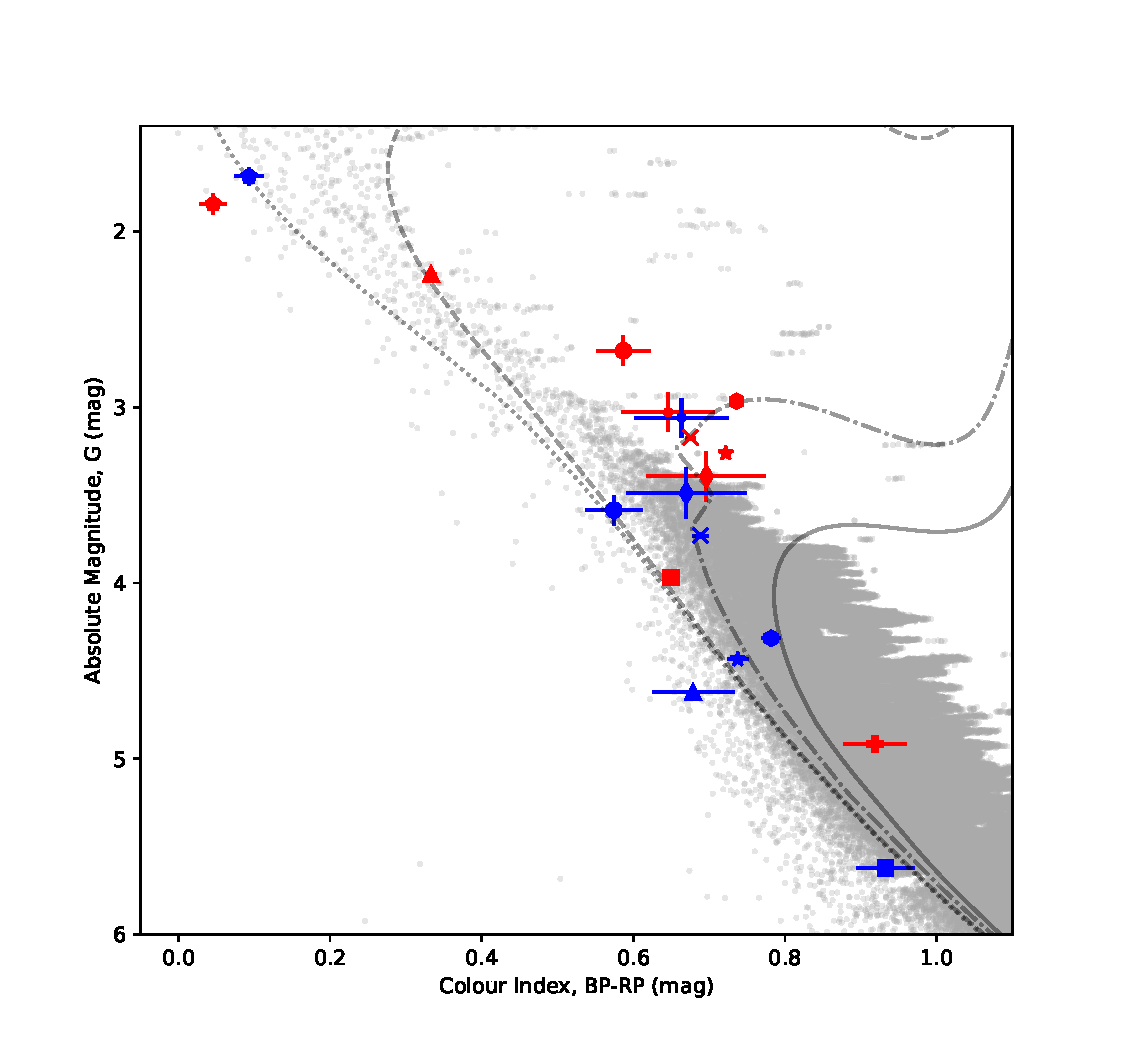
\includegraphics[width=\linewidth]{HRD}
    \caption{The two colours, red and blue, represent primary and secondary components respectively. These symbols represent EBs: TIC279087522 ($\pentagonblack$), TIC30122338 ($\mdblkcircle$), TIC7695666 ($\times$), TIC66602813 ($\mdblksquare$), TIC63579446 ($\bigstar$), TIC201497357 ($\blacktriangle)$, TIC349480507 ($\cdot$), TIC349059354 ($\mdblkdiamond$), TIC78568736 ($+$; secondary outside figure boundaries), TIC80556181 ($\varhexagonblack$). Isochrones from \citet{Dotter16,Choi16,Paxton18} represent stellar ages $0.5 - 10 \mathrm{\ Gyr}$ from left to right. Main sequence stars (grey) are from \citet{Gaia18}}.
    \label{fig:CMD}
\end{figure}

\section{Conclusion}\label{sec:Conclusion}
% This project was highly successful in finding multiple benchmark candidates for PLATO which are consistent with the parameters set by the mission. Our best candidates are TIC279087522, TIC63579446, TIC349059354 and TIC201497357. These are mainly solar-type stars which are low in magnitude ($4<G<5$), meaning this project was successful in attaining our aim and finding good benchmark candidates.

This project was successful in finding multiple benchmark candidates for calibration of PLATO which are consistent with the parameters set by the mission, fulfilling the aim. Our best candidates are TIC7695666, TIC349480507 and TIC80556181. These exhibit properties $\sim 1 \ M_{\odot}$ and $V<11\mathrm{\ mag}$. We therefore recommend these stars for further study. 

\begin{acknowledgments}
% This work has made use of data from the European Space Agency (ESA) mission
% {\it Gaia} (\url{https://www.cosmos.esa.int/gaia}), processed by the {\it Gaia}
% Data Processing and Analysis Consortium (DPAC,
% \url{https://www.cosmos.esa.int/web/gaia/dpac/consortium}). Funding for the DPAC
% has been provided by national institutions, in particular the institutions
% participating in the {\it Gaia} Multilateral Agreement.\\

% Some of the data presented in this paper were obtained from the Mikulski Archive for Space Telescopes (MAST). STScI is operated by the Association of Universities for Research in Astronomy, Inc., under NASA contract NAS5-26555. Support for MAST for non-HST data is provided by the NASA Office of Space Science via grant NNX13AC07G and by other grants and contracts. 
\end{acknowledgments}
%% To help institutions obtain information on the effectiveness of their 
%% telescopes the AAS Journals has created a group of keywords for telescope 
%% facilities.
%
%% Following the acknowledgments section, use the following syntax and the
%% \facility{} or \facilities{} macros to list the keywords of facilities used 
%% in the research for the paper.  Each keyword is check against the master 
%% list during copy editing.  Individual instruments can be provided in 
%% parentheses, after the keyword, but they are not verified.

\vspace{5mm}
\facilities{MAST (TESS), Gaia (DR3)}

%% Similar to \facility{}, there is the optional \software command to allow 
%% authors a place to specify which programs were used during the creation of 
%% the manuscript. Authors should list each code and include either a
%% citation or url to the code inside ()s when available.

\cprotect\software{\verb|jktebop| v43 \citep{Southworth13}, \verb|Lightcurve| v2.5.0 \citep{Lightkurve18}
%, \verb|Astropy| v6.1.4 \citep{Astropy13,Astropy18,Astropy20}
}

%% Appendix material should be preceded with a single \appendix command.
%% There should be a \section command for each appendix. Mark appendix
%% subsections with the same markup you use in the main body of the paper.

%% Each Appendix (indicated with \section) will be lettered A, B, C, etc.
%% The equation counter will reset when it encounters the \appendix
%% command and will number appendix equations (A1), (A2), etc. The
%% Figure and Table counter will not reset.

% \appendix

% \appendix

%% For this sample we use BibTeX plus aasjournals.bst to generate the
%% the bibliography. The sample631.bib file was populated from ADS. To
%% get the citations to show in the compiled file do the following:
%%
%% pdflatex sample631.tex
%% bibtext sample631
%% pdflatex sample631.tex
%% pdflatex sample631.tex

\bibliography{main}{}
\bibliographystyle{aasjournal}

%% This command is needed to show the entire author+affiliation list when
%% the collaboration and author truncation commands are used.  It has to
%% go at the end of the manuscript.
%\allauthors

%% Include this line if you are using the \added, \replaced, \deleted
%% commands to see a summary list of all changes at the end of the article.
%\listofchanges

\end{document}

% End of file `sample631.tex'.
